\documentclass[11 pt]{article} 
\usepackage[left=2cm, top=2cm, right=2cm, bottom=2.5cm, footskip=.5cm]{geometry}
\usepackage{graphicx}
\usepackage{subcaption} 
\usepackage{subfig}
\usepackage{amsmath}
\usepackage{url}
\usepackage{booktabs}
\usepackage{units}
\usepackage{enumitem}
\usepackage{listings}
\usepackage{float}
\usepackage{booktabs}
%\usepackage{hyperref}

\author{Natalia Zuniga-Garcia}
\title{Exercises 2 Online Learning}
\date{September 27, 2017}

\begin{document}

\maketitle

\section{Stochastic gradient descent: background}

In the previous set of exercises, we learned about gradient descent.  To review: suppose we have a loss function $l(\beta)$ that we want to minimize, like a negative log likelihood or negative log posterior density.  In gradient descent, we start with an initial guess $\beta^{(0)}$ and then repeatedly take steps in a downhill direction:
$$
\beta^{(t+1)} = \beta^{(t)} - \gamma^{(t)} g^{(t)} \, ,
$$
where $g^{(t+1)}  = \nabla l(\beta^{(t)})$ is the gradient of the loss function evaluated at the previous iterate, which points locally uphill, and where $ \gamma^{(t)}$ is a scalar step size (which might or might not actually depend on the iteration number $t$).

To calculate the gradient, we need to sum over the contributions from all $n$ data points.  But what if instead $g^{(t)}$ were not the actual gradient of the loss function, but merely an approximation to that gradient?  In this context, by an approximation, we mean that the (negative) step direction $g^{(t)}$ is a random variable that satisfies
$$
E(g^{(t)}) = \nabla l(\beta^{(t)}) \, .
$$
Thus $g^{(t)}$ is an unbiased estimate of the gradient, but has some error.   If you used such a random $g^{(t)}$ in your update instead of the actual gradient, some individual steps would lead you astray, but each step would take you in the right direction, on average.  This is called \textit{stochastic gradient descent,} or SGD. 

Does SGD actually converge to the minimum of $l(x)$?  It's easy to convince yourself that, if your step sizes $\gamma^{(t)}$ were constant, then you'd never get to the minimum.  You might get close, but the randomness in the search directions would have you perpetually bouncing around the minimum like a moth around a flame.  It follows that, if you ever hope to get to the minimum, a necessary condition is that your step sizes $\gamma^{(t)}$ get smaller, at least on average.

So assuming you handle the step sizes properly---a big if, as we'll see---here are two follow-up questions.
\begin{enumerate}
	\item How random can these $g^{(t)}$'s be and still end up getting us to minimum of $l(\beta)$? 
	\item Why on earth would we want to inject randomness into the gradient-descent direction in the first place?
\end{enumerate}

The answers are: 1) pretty darn random, and 2) so that we only ever have to touch one data point at a time!  Let's explore.


\newpage

\section{SGD for logistic regression}

\begin{enumerate}[label=(\Alph*)]
	
	\item Let $l(\beta)$ be the negative log likelihood associated with the logistic regression model, which was a sum over $n$ terms (one term for each data point).  Earlier you derived the gradient of $l(\beta)$.  If you haven't already, show that this gradient can be written in the form
	$$ 	\nabla l(\beta) =  \sum_{i=1}^n g_i(\beta)  $$
	$$ g_i(\beta) = (\hat y_i - y_i) x_i $$
	$$ \hat{y}_i = E(y_i \mid \beta) = m_i \cdot w_i(\beta) = m_i \cdot \frac{1}{1 + \exp(-x_i^T \beta)} \, $$
	
	\vspace{2mm}
	\textbf{Solution}

In Exercise 1, Part 2A, we showed that:

 $$  \nabla l(\beta)  = \displaystyle\sum_{i=1}^{N}\left \{ (m_iw_i - y_i)x_i \right \}$$	
 
 Thus, we can state:
 
 $$ g_i(\beta) =  (m_iw_i - y_i)x_i  $$
 
 Where we know that $m_iw_i$ is the fitted value of $y_i$ for a given $\beta$. So  $\hat y_i = m_iw_i$, 
 
 $$	\hat{y}_i = E(y_i \mid \beta) = m_i \cdot w_i(\beta) = m_i \cdot \frac{1}{1 + \exp(-x_i^T \beta)} $$
 
 Then, we can probe that:
 
  $$ g_i(\beta) =  (\hat y_i - y_i)x_i  $$
 
 
	
	
	
	\newpage
	
	\item Optional but interesting.  Suppose that you draw a single data point at random from your sample, giving you the pair $\{y_i, x_i\}$.  If you can, show that the random vector $n g_i(\beta)$ is an unbiased estimate of $\nabla l(\beta)$:
	$$
	E \{ n g_i(\beta) \} = \nabla l(\beta) \, ,
	$$
	where the expectation is under random sampling from the set of all $\{y_i, x_i\}$ pairs.  Alternatively, you can also show that these two vectors have the same expectation under the assumption that all the $\{y_i, x_i\}$ pairs are drawn $i.i.d.$ from some wider population distribution $\Pi$.
	
	Note: when we apply SGD using this fact, we typically drop the leading term of $n$ in front of $g_i(\beta)$ and absorb it implicitly into the step size $\gamma^{(t)}$.
	
	
	\vspace{2mm}
	\textbf{Solution}
	
	We have a single data point at random given the pair $\{y_i, x_i\}$, where n is constant so we have:
	$$	E \{ n g_i(\beta) \} = n E \{g_i(\beta) \} $$
	For a discrete random variable, the expected value is calculated by summing the product of the value of the random variable and its associated probability. We know that $i$ is random, selected at random draw, and it follows a uniform distribution such that for j={1,2,..,n}:
	$$ P(i=j)= \frac{1}{n} $$
	So we can write the expectation as:
	$$	E \{ n g_i(\beta) \} =  n \bigg[\sum_{i=1}^n g_i(\beta) P(i=j)  \bigg] = n \bigg[\frac{1}{n}\sum_{i=1}^n g_i(\beta)   \bigg] = n \bigg[\frac{1}{n}\nabla l(\beta)\bigg]= \nabla l(\beta) $$
	So we probed that:
	$$	E \{ n g_i(\beta) \} = \nabla l(\beta)$$
	
	
	
	
	
	\newpage
	
	
	\item For the rest of the exercises, you can take the claim in (B) as given.  The idea here is that, instead of using the gradient calculated from all $n$ data points to choose our step direction in gradient descent, we use the gradient $g_i(\beta$) calculated from a single data point, sampled randomly from the whole data set.  Because this single-data-point gradient is an unbiased estimate of the full-data gradient, we move in the right direction toward the minimum, on average.
	
	Try this out!  That is, code up stochastic gradient descent for logistic regression, in which each step takes the form
	$$
	\beta^{(t+1)} = \beta^{(t)} - \gamma^{(t)} g_t (\beta^{(t)}) \, ,
	$$
	where $g_t (\beta)$ is the gradient contribution from single randomly sampled data point, evaluated at the current guess for $\beta$.
	
	Some notes:
	\begin{enumerate}[label=\arabic*.]
		\item Focus on functionality first.  Forget about speed for now.  It's said in CS that premature optimization is the root of all evil.  Don't worry: soon enough, you'll have an SGD implementation that will blaze.
		\item You'll almost certainly want to try this on simulated data first, so you can compare the answer you get both with the ground truth and with the answer you get from something like Newton's method.  Simply plotting truth versus SGD estimate, or Newton estimate versus SGD estimate, will be informative.
		\item For this part,  keep the step size constant over time: that is, $\gamma^{(t)} \equiv \gamma$.  You'll want to start your debugging process with $\gamma$ pretty small.  (For perspective, $\gamma = 1$ is considered a big step size).  A good step size will depend very much on your data, but if things are going crazy, go an order of magnitude smaller, i.e.~from 0.1 to 0.01 or even smaller.  This doesn't have to be elegantly handled in your code (i.e.~you can hard-code it), because you won't be using a constant step size going forward---it's just for intuition-building here.
		\item Once you feel like your code is doing something vaguely reasonable, start experimenting with the step size $\gamma$.  Note any general lessons you learn.
		\item Sampling can be with or without replacement.  However, it can easily be the case that you need more SGD steps than there are samples $n$ in the data set, implying that if you sample without replacement, you'll have to start over (but not reset $\beta$!) after $n$ samples.   That's OK!  Sometimes a batch of $n$ SGD steps, sampled without replacement from the full data set---which is just a permutation of the original data points---is called a \textit{training epoch}.  (Prompting the question: epic training or training epoch?)
	\end{enumerate}
	
	
	You'll also want to track the convergence of the algorithm.  Some notes on this point as you think through your options:
	\begin{enumerate}[label=\arabic*.]
		\item The surefire way to do this is to track the value of the full objective function $l(\beta)$ at every step, so you can plot it over time and check whether it's actually going down.
		\item Of course, if you do this, you'll defeat the purpose of touching only one data point at every iteration.  You'll probably want to do it anyway for now, as you build intuition and debug code.  But you should also consider tracking something that doesn't suffer from this problem: the running average of $l_t(\beta)$, the individual log likelihood contribution from the data point you sample at step $t$.  Although.~.~.~.
		\item Really, if you want to be even more clever than this, you can track the exponentially weighted moving average\footnote{\url{https://en.wikipedia.org/wiki/Moving_average#Exponential_moving_average}} of the $l_t(\beta)$'s, so that the influence of the early (bad) log-likelihood evaluations decays over time. 
		
	\end{enumerate}
	\newpage
	\vspace{2mm}
	\textbf{Solution}
	
	The functions\footnote{The solution is presented in the file $solution02-SDS385RCode.Rmd$} are shown as follow,
	
	
	\begin{lstlisting}[language=R]
	
# Function 1. Estimate the Success Probability
wi.estimate <- function(b, X){
# Inputs:
# b regression parameter P x 1
# X Matrix of features N x P
# Output:
# wi Sucess Probability N x 1

w <- 1/(1+exp(-X %*% b)) 
w = pmax(w, 1E-6); w = pmin(w, 1-1E-6); 
return(w)
}

# Function 2. Estimate the negative log likelihood
Negll <- function(b, y, X, m){
# Input:
# b regression parameter P x 1
# y vector of response N x 1
# X Matrix of features N x P
# m number of trial for the ith case
# Output:
# Negative log likelihood of binomial distribution

ll <- -sum(dbinom(y, m, wi.estimate(b, X), log = TRUE))
return(ll)
}

# Function 3. Estimate the gradient of the negative log likelihood
Gradll <- function(b, y, X, m){
# Input:
# b regression parameter P x 1
# y vector of response N x 1
# X Matrix of features N x P
# m number of trial for the ith case
# Output:
# gradient of l(b) P x 1

grad.ll <- as.numeric(y - m * wi.estimate(b, X)) * X
return(-colSums(grad.ll))
}




# Function 4. Stochastic Gradient Descend 
SGradDes <- function(y, X, beta, m, iter, epsilon, alpha){
# Input:
# y vector of response N x 1
# X Matrix of features N x P
# beta: initial guees of beta P x 1
# m: number of trial for the ith case
# iter: maximum iterations allowed if it doesn't converge
# epsilon: minimum error allowed for convergency creteria
# alpha: step size (gamma based on class document)
# Output:
# Negative log likelihood per iteration
# Using stochastic gradient descend
# b regression parameter P x 1

# Initial Iteration (GUESS)
betas = array(NA, dim=c(iter, ncol(X)))
betas[1,] = beta
ll = array(NA, dim = iter)
ll[1] = Negll(betas[1,], y, X, m)

# Iterations
for (i in 2:iter){
r <- sample(nrow(X), 1) # Draw a random sample with replacement
grad <- Gradll(betas[i-1,], matrix(y[r], nrow=1), matrix(X[r,], nrow=1), m)

# Gradient Descend
betas[i,] <- betas[i-1,] - alpha * grad 
ll[i] <- Negll(betas[i,], y, X, m)
# Note that I am tracking the full objective function in every step
# Thus I am not touching only one point per iteration as SGD intended
# I'm doing this with the objective of develop a learning process for myself

# Checking for Convergence
error = abs((ll[i] - ll[i-1])/(ll[i-1] + epsilon))
if (error < epsilon){
cat('Stochastic Gradient Descend has converged in iterations:',i)
ll <- ll[1:i]
betas <- betas[1:i,]
break;
} else if (i == iter && error >= epsilon){
print('Stochastic Gradient Descend has not converged')
break;
}
}
return(list("Negll" = ll, "beta" = betas[i,]))
}

	\end{lstlisting}
	
	\vspace{5mm}
	The implemented function is evaluated using the $wdbc$ database used in Exercise 1 Part 2. The results of the objective function are shown in Figure \ref{fig:Fig1}, I experimented different step size ($\gamma$) values. We can observe that for low $\gamma$ values,  the objective function decay slowly. While, for high $\gamma$ values, the objective function decay quickly. However, if the $\gamma$ is high (for instance $\gamma=1$) the algorithm does not converge and it tends to variate significantly, as shown in Figure \ref{fig:Fig1} part (f).

\begin{figure}[H]
	\begin{center}
		\begin{subfigure}[h]{0.45\linewidth}
			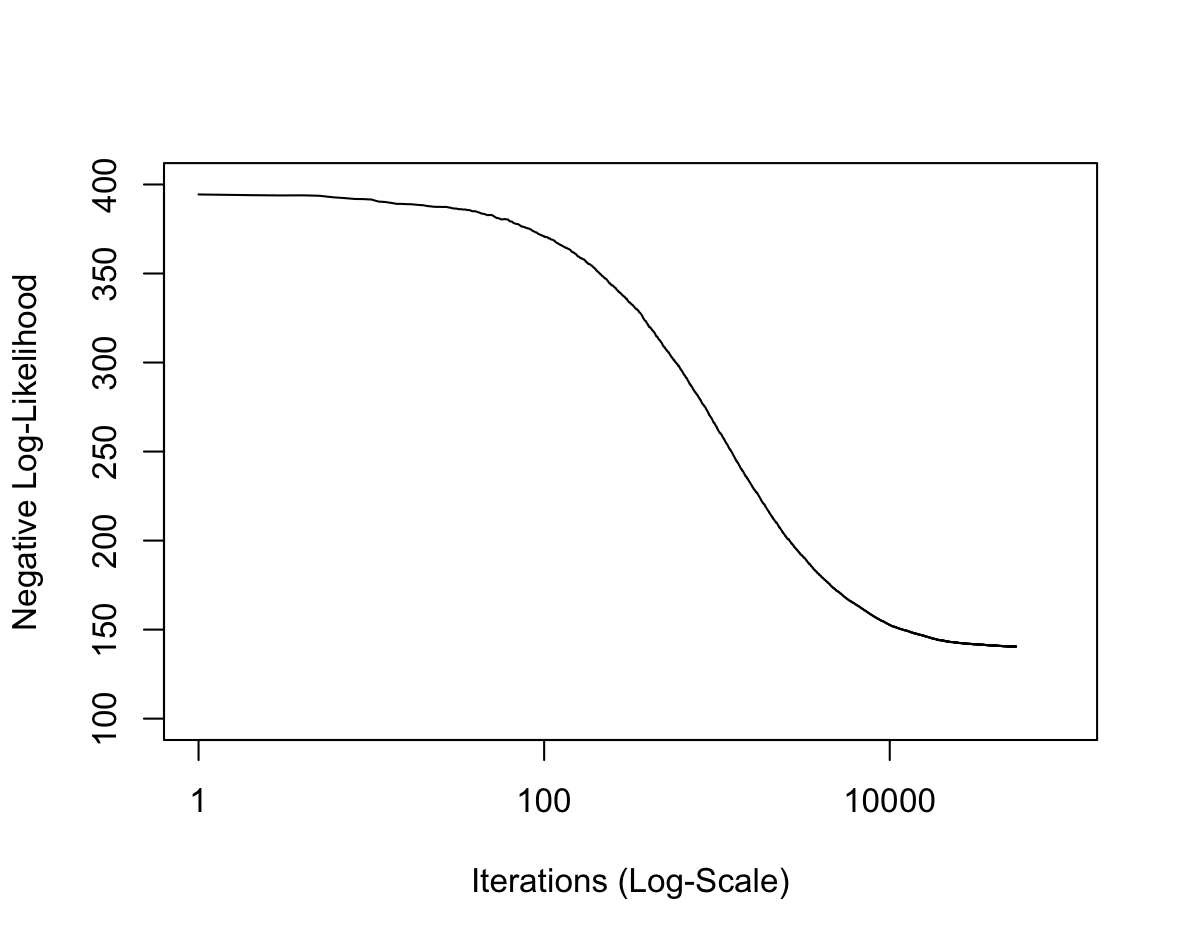
\includegraphics[width=\linewidth]{Fig/F1PC0001.png}
			\caption{Step size $\gamma=0.001$}
		\end{subfigure}
		\begin{subfigure}[h]{0.45\linewidth}
			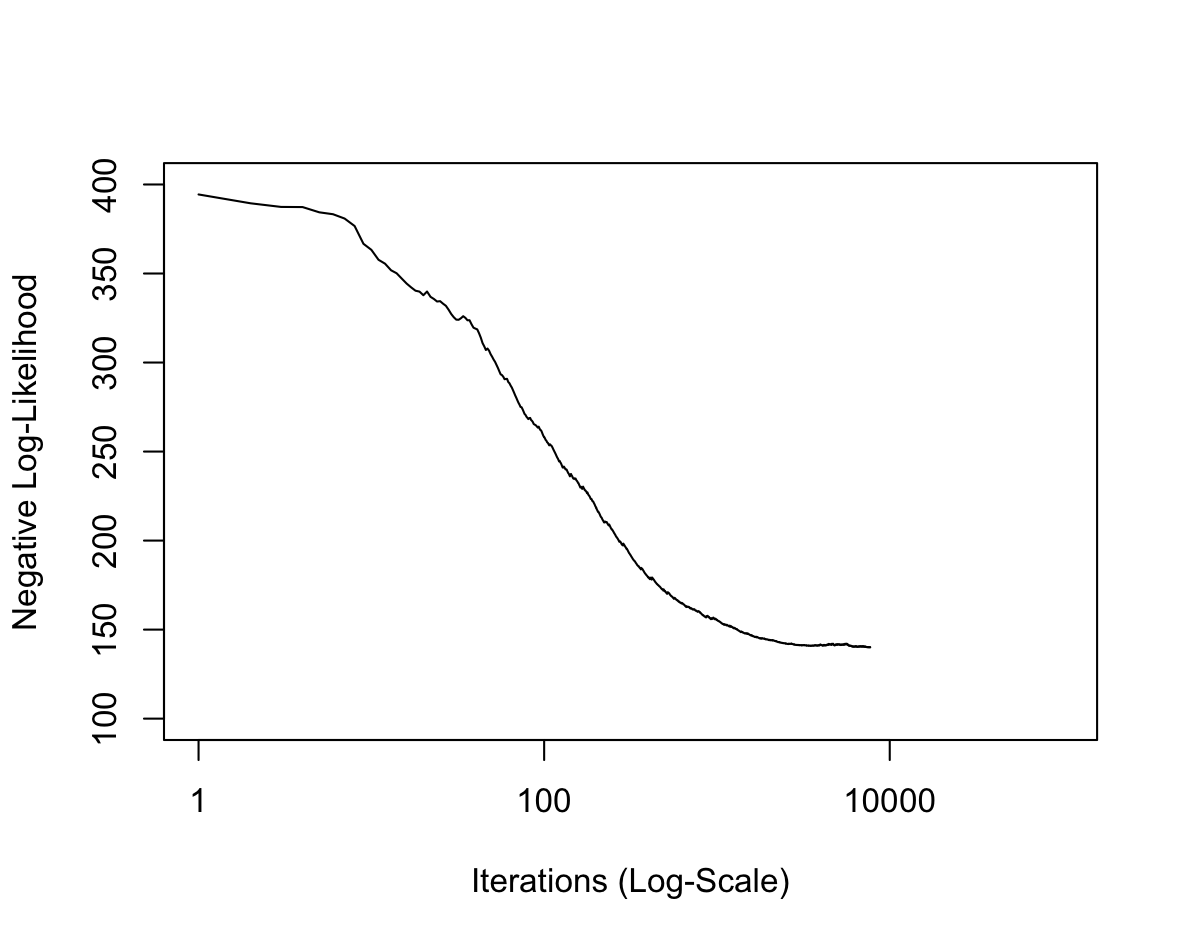
\includegraphics[width=\linewidth]{Fig/F1PC001.png}
			\caption{Step size $\gamma=0.01$}
		\end{subfigure}
		\begin{subfigure}[h]{0.45\linewidth}
			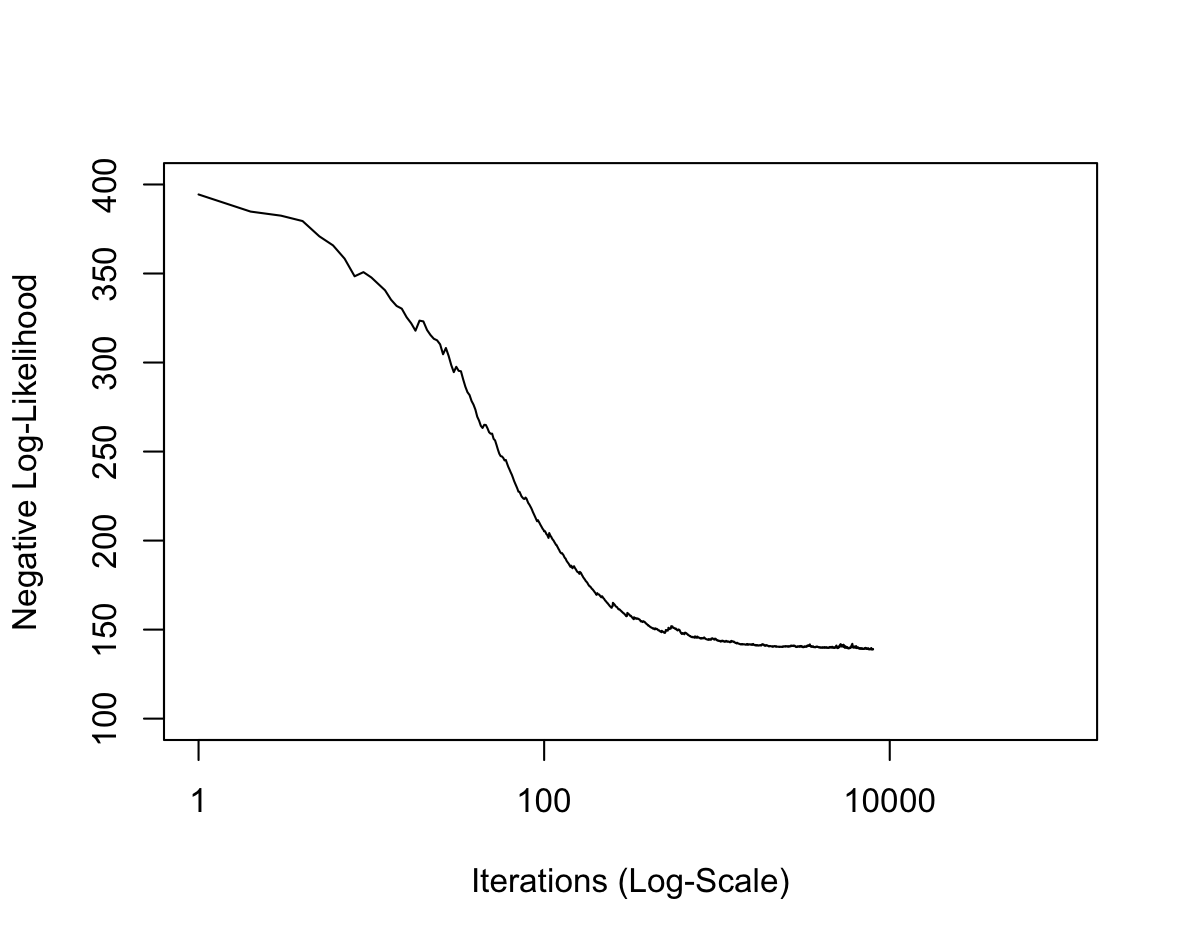
\includegraphics[width=\linewidth]{Fig/F1PC0025.png}
			\caption{Step size $\gamma=0.025$}
		\end{subfigure}
		\begin{subfigure}[h]{0.45\linewidth}
			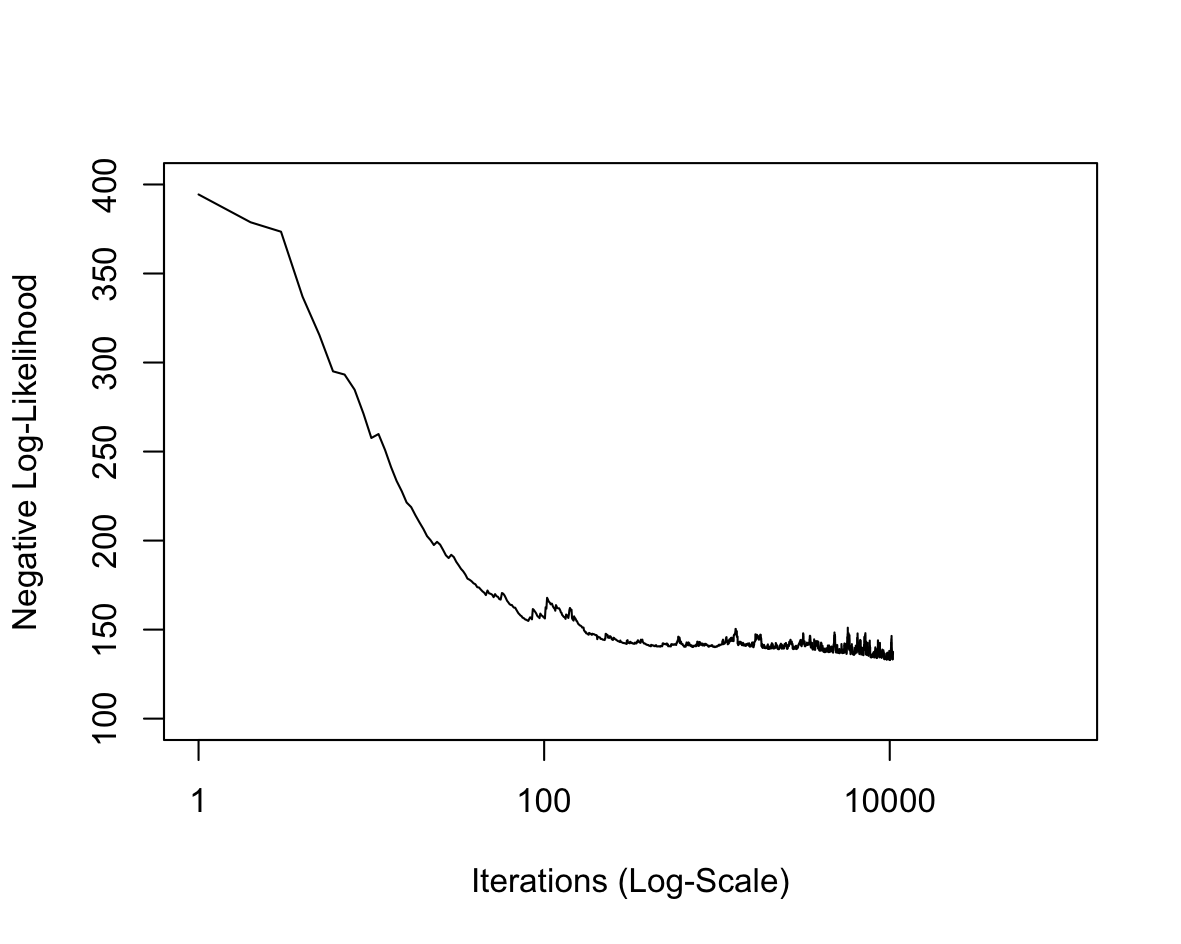
\includegraphics[width=\linewidth]{Fig/F1PC01.png}
			\caption{Step size $\gamma=0.1$}
		\end{subfigure}
		\begin{subfigure}[h]{0.45\linewidth}
			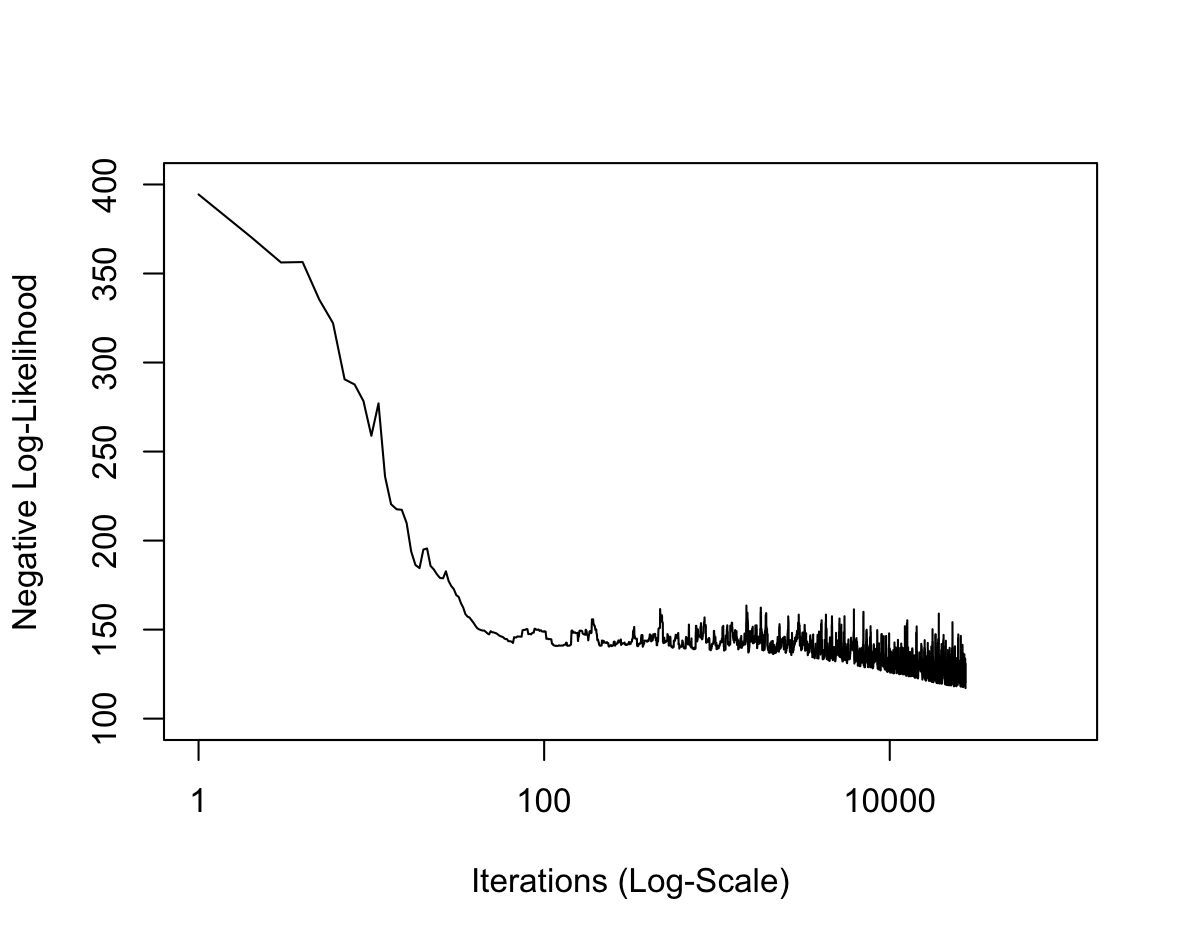
\includegraphics[width=\linewidth]{Fig/F1PC025.png}
			\caption{Step size $\gamma=0.25$}
		\end{subfigure}
		\begin{subfigure}[h]{0.45\linewidth}
			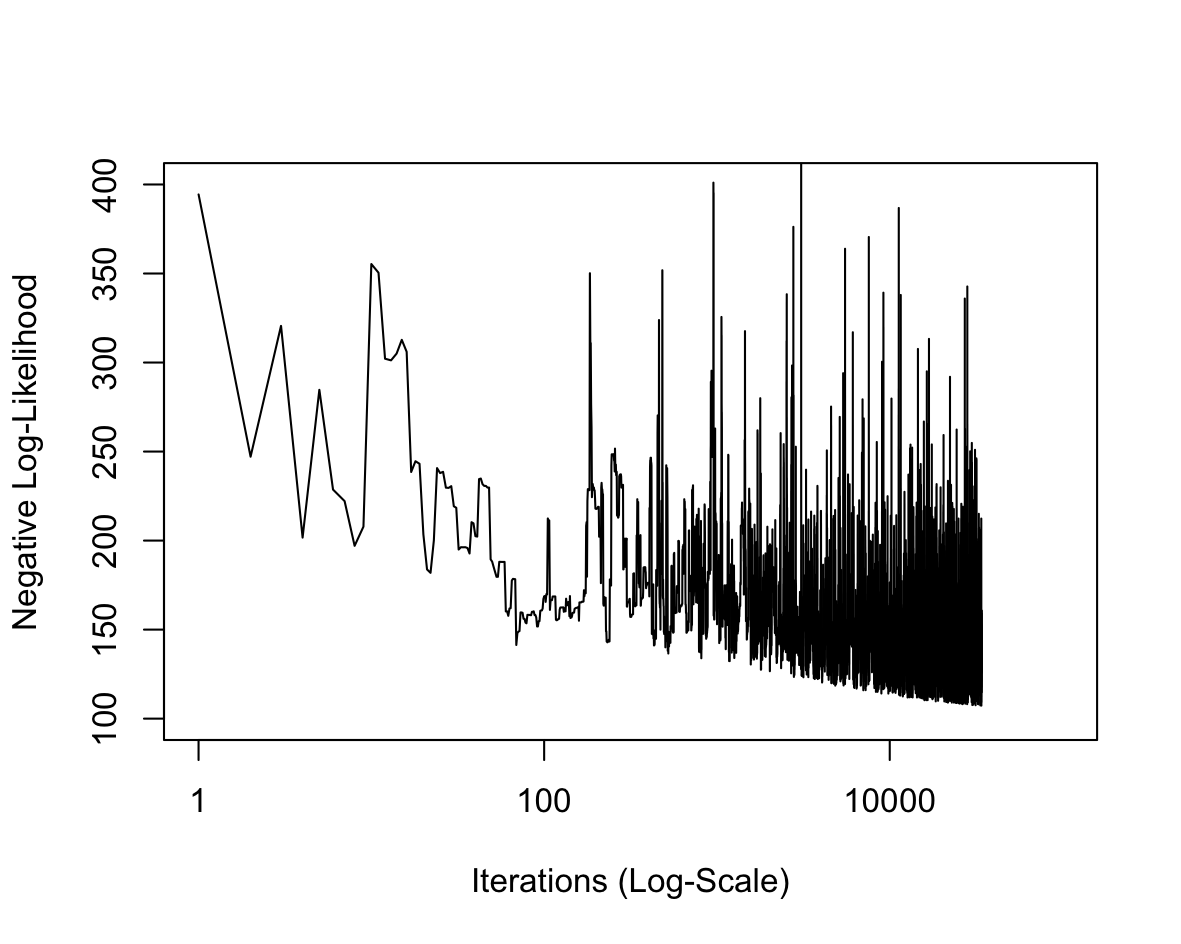
\includegraphics[width=\linewidth]{Fig/F1PC1.png}
			\caption{Step size $\gamma=1$}
		\end{subfigure}
		\caption{Stochastic Gradient Descent - experimenting with step size $\gamma$}
		\label{fig:Fig1}
	\end{center}
\end{figure}

	
	\newpage
	
	\item Now try a decaying step size.  Specifically, use the Robbins--Monro\footnote{\url{https://en.wikipedia.org/wiki/Stochastic_approximation}} rule for step sizes: 
	$$
	\gamma^{(t)} = C (t + t_0)^{-\alpha} \, ,
	$$
	where $C > 0$, $\alpha \in [0.5, 1]$, and $t_0$ (the ``prior number of steps'') are constants.  The exponent $\alpha$ is usually called the learning rate.  Clearly the closer $\alpha$ is to 1, the more rapidly the step sizes decay.
	
	Implement the Robbins-Monro rule in your SGD code. Pick a smallish $t_0$ (1 or 2) and run with it.   Fiddle around with $C$ and $\alpha$ to see if you can get good performance. 
	
	\vspace{2mm}
	\textbf{Solution}
	
	The function\footnote{The solution is presented in the file $solution02-SDS385 RCode.Rmd$} is:
	
	\begin{lstlisting}[language=R]

# Function 5. Stochastic Gradient Descend Decaying Step Size
SGradDesRM <- function(y, X, beta, m, iter, epsilon, C, t, alpha){
# Input:
# y vector of response N x 1
# X Matrix of features N x P
# beta: initial guees of beta P x 1
# m: number of trial for the ith case
# iter: maximum iterations allowed if it doesn't converge
# epsilon: minimum error allowed for convergency creteria
# C: constant in the Robbins-Monro rule
# t: t0 prior number of steps Robbins-Monro rule
# alpha: learning rate Robbins-Monro rule
# Output:
# Negative log likelihood per iteration
# Using stochastic gradient descend
# with decaying step size
# b regression parameter P x 1

# Initial Iteration (GUESS)
betas = array(NA, dim=c(iter, ncol(X)))
betas[1,] = beta
ll = array(NA, dim = iter)
ll[1] = Negll(betas[1,], y, X, m)

# Iterations
for (i in 2:iter){
r <- sample(nrow(X), 1) # Draw a random sample with replacement
grad <- Gradll(betas[i-1,], matrix(y[r], nrow=1), matrix(X[r,], nrow=1), m)

# Gradient Descend
step <- C*(i+t)^(-alpha) # Robbins-Monro rule
betas[i,] <- betas[i-1,] - step * grad 
ll[i] <- Negll(betas[i,], y, X, m)

# Checking for Convergence
error = abs((ll[i] - ll[i-1])/(ll[i-1] + epsilon))
if (error < epsilon){
cat('Stochastic Gradient Descend has converged in iterations:',i)
ll <- ll[1:i]
betas <- betas[1:i,]
break;
} else if (i == iter && error >= epsilon){
print('Stochastic Gradient Descend has not converged')
break;
}
}
return(list("Negll" = ll, "beta" = betas[i,]))
}	

	\end{lstlisting}
	
	\vspace{5mm}
	Similarly, the implemented function is evaluated using the $wdbc$ database. The results of the objective function are shown in Figure \ref{fig:Fig2} and \ref{fig:Fig3}, where I experimented different $C$ and $\alpha$ values, respectively. \\
	We can observe that when we increase the value of  $C$ (Figure \ref{fig:Fig2}), the objective function decrease faster but present some variations. While for low values of $C$, it decays slowly and smoother.\\
	On the other hand, when we increase the value of the learning rate $\alpha$, the objective function decays slower. This result could be because at higher $\alpha$ values, the step size decays quickly, thus, the convergence is slower. 
	
	
	\begin{figure}[H]
		\begin{center}
			\begin{subfigure}[h]{0.45\linewidth}
				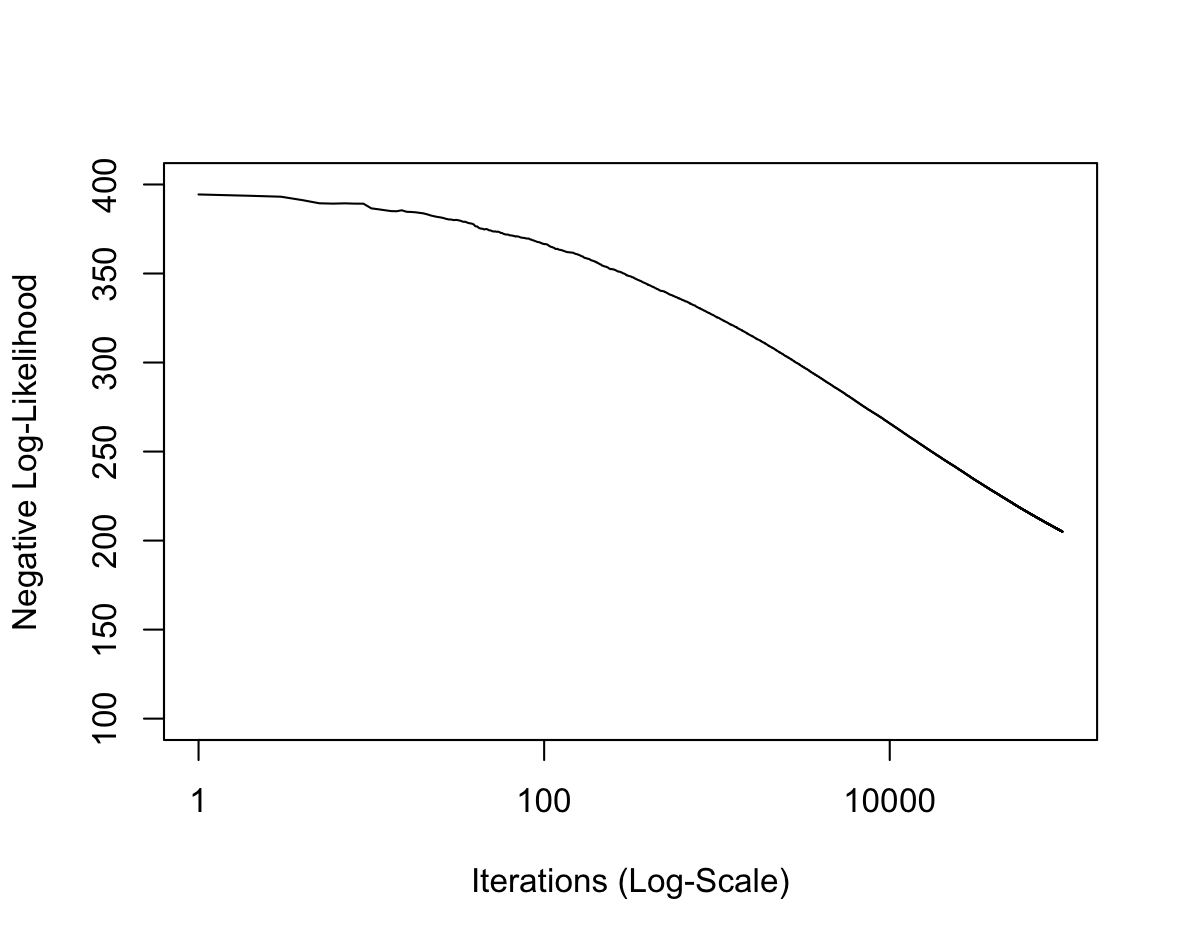
\includegraphics[width=\linewidth]{Fig/F2PD001.png}
				\caption{$C=0.01$}
			\end{subfigure}
			\begin{subfigure}[h]{0.45\linewidth}
				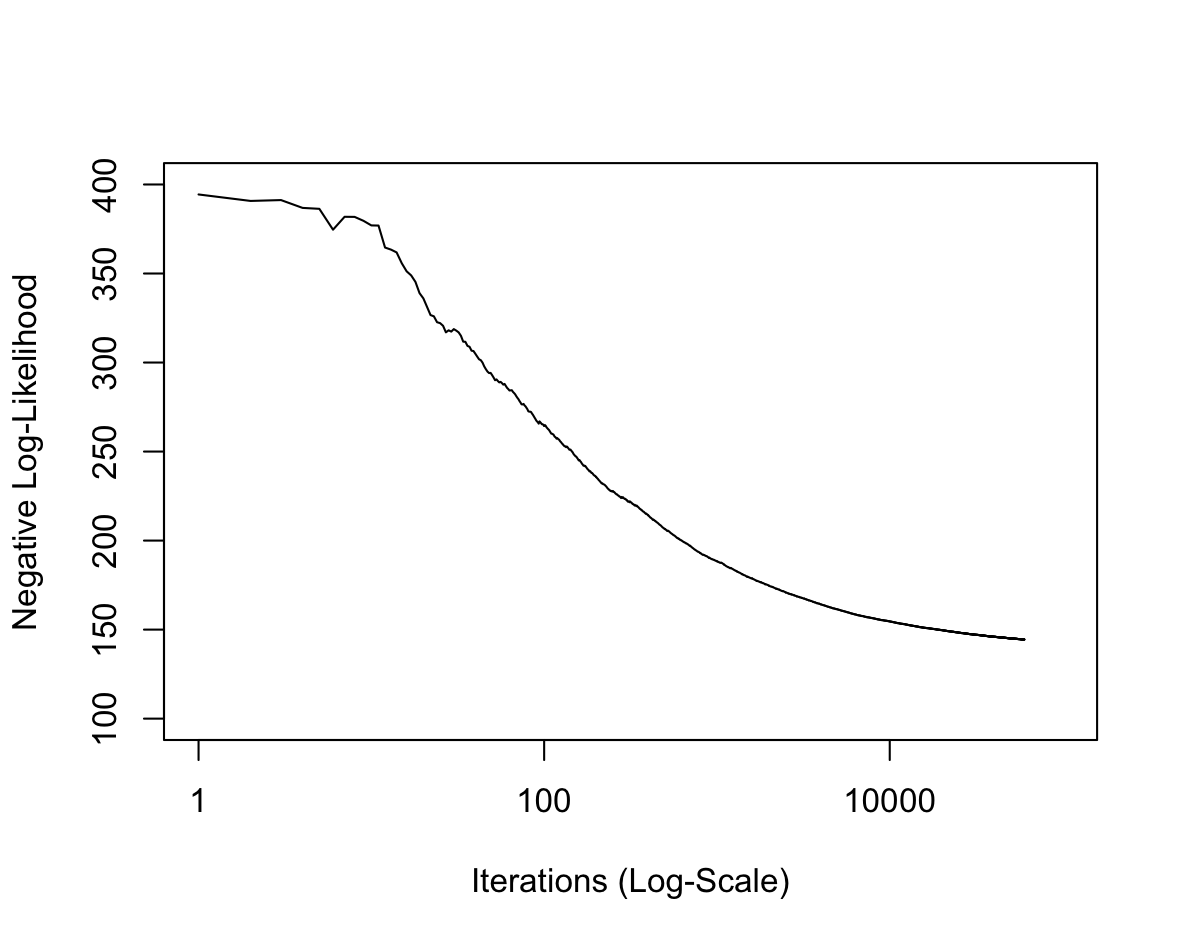
\includegraphics[width=\linewidth]{Fig/F2PD01.png}
				\caption{$C=0.1$}
			\end{subfigure}
			\begin{subfigure}[h]{0.45\linewidth}
				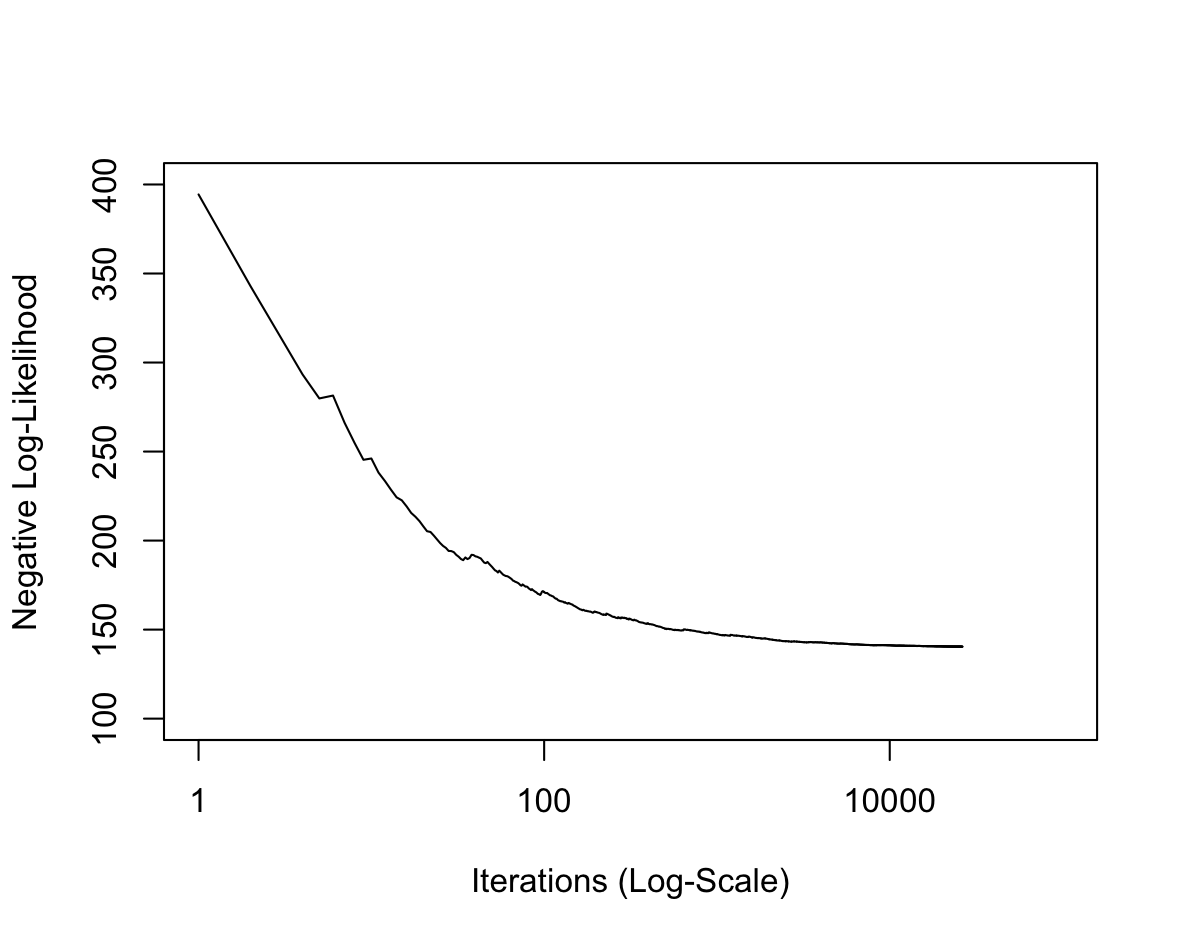
\includegraphics[width=\linewidth]{Fig/F2PD04.png}
				\caption{$C=0.4$}
			\end{subfigure}
			\begin{subfigure}[h]{0.45\linewidth}
				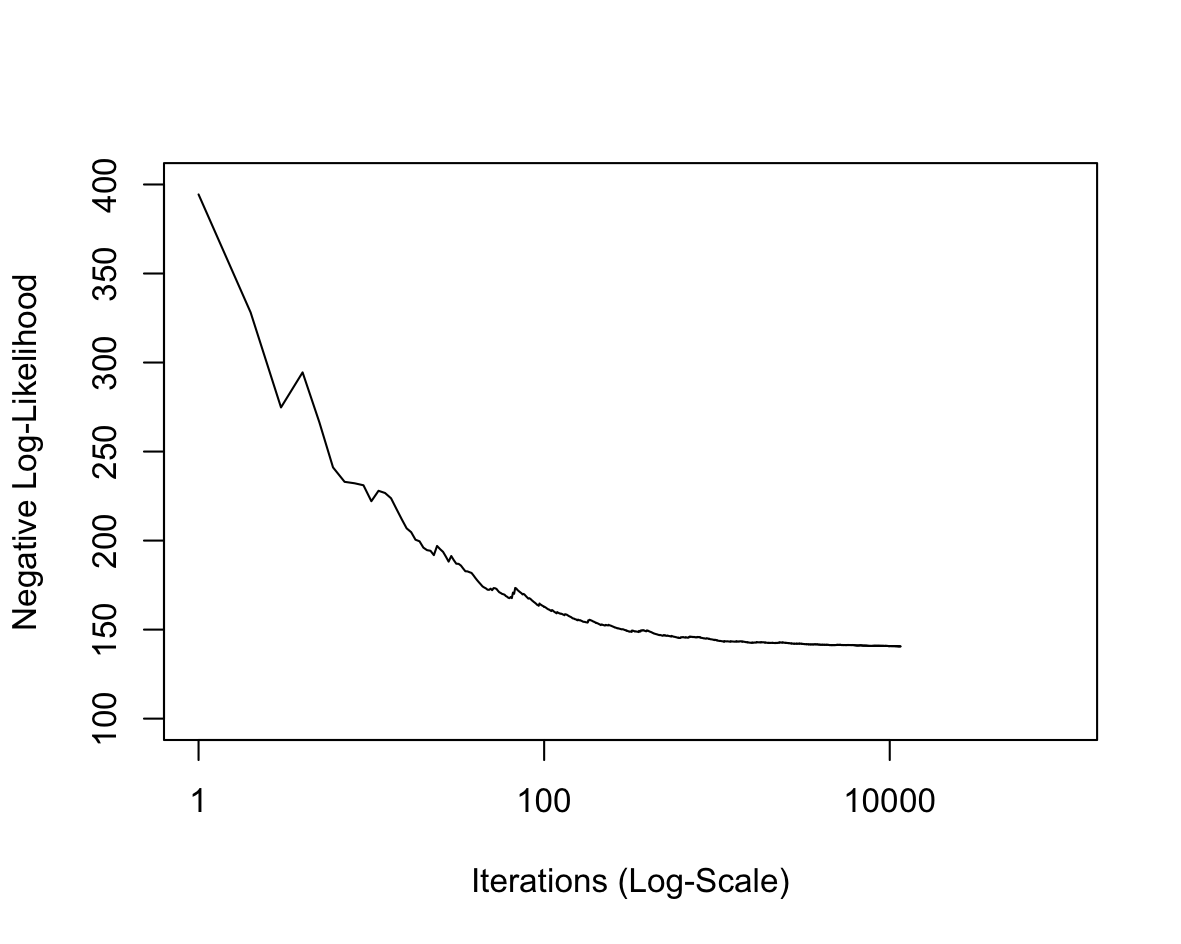
\includegraphics[width=\linewidth]{Fig/F2PD06.png}
				\caption{$C=0.6$}
			\end{subfigure}
			\begin{subfigure}[h]{0.45\linewidth}
				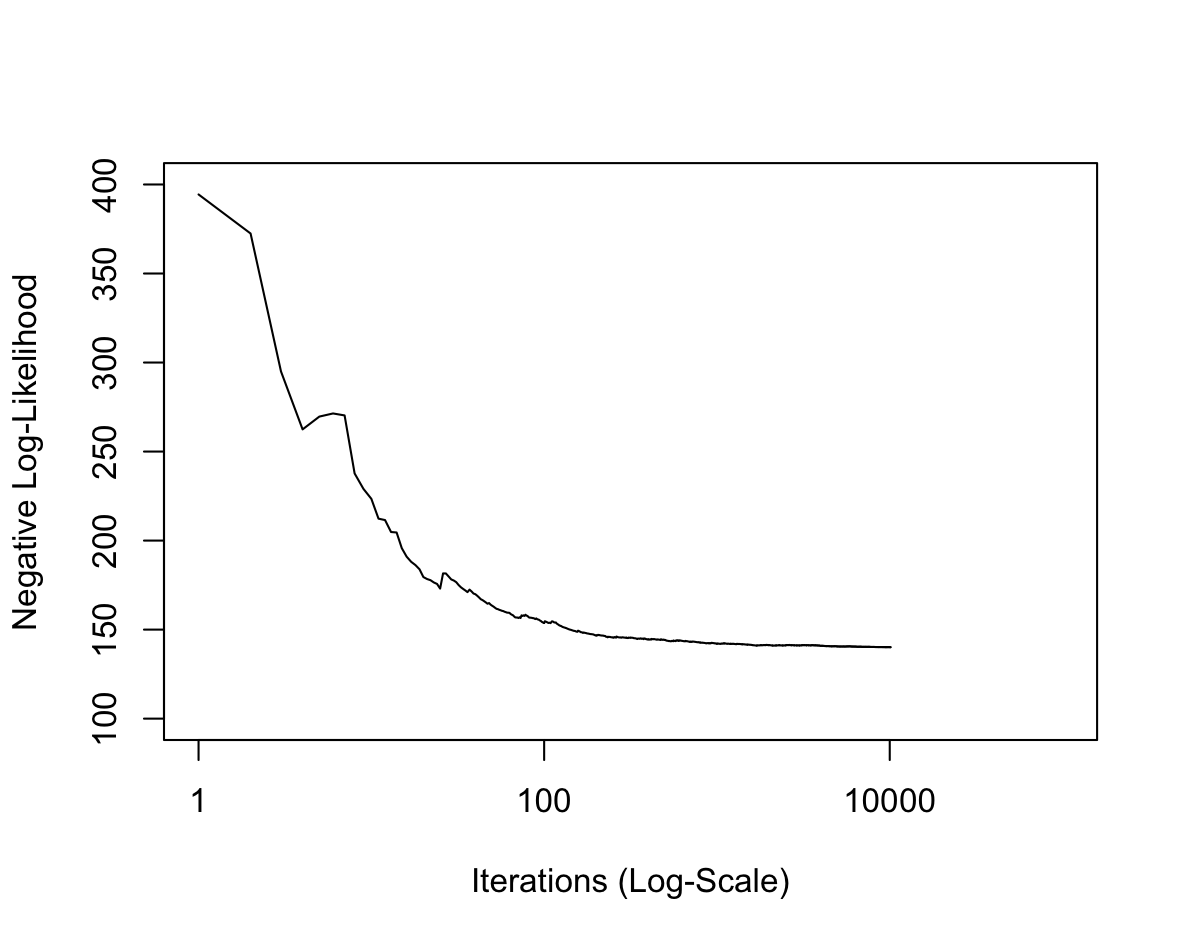
\includegraphics[width=\linewidth]{Fig/F2PD08.png}
				\caption{$C=0.8$}
			\end{subfigure}
			\begin{subfigure}[h]{0.45\linewidth}
				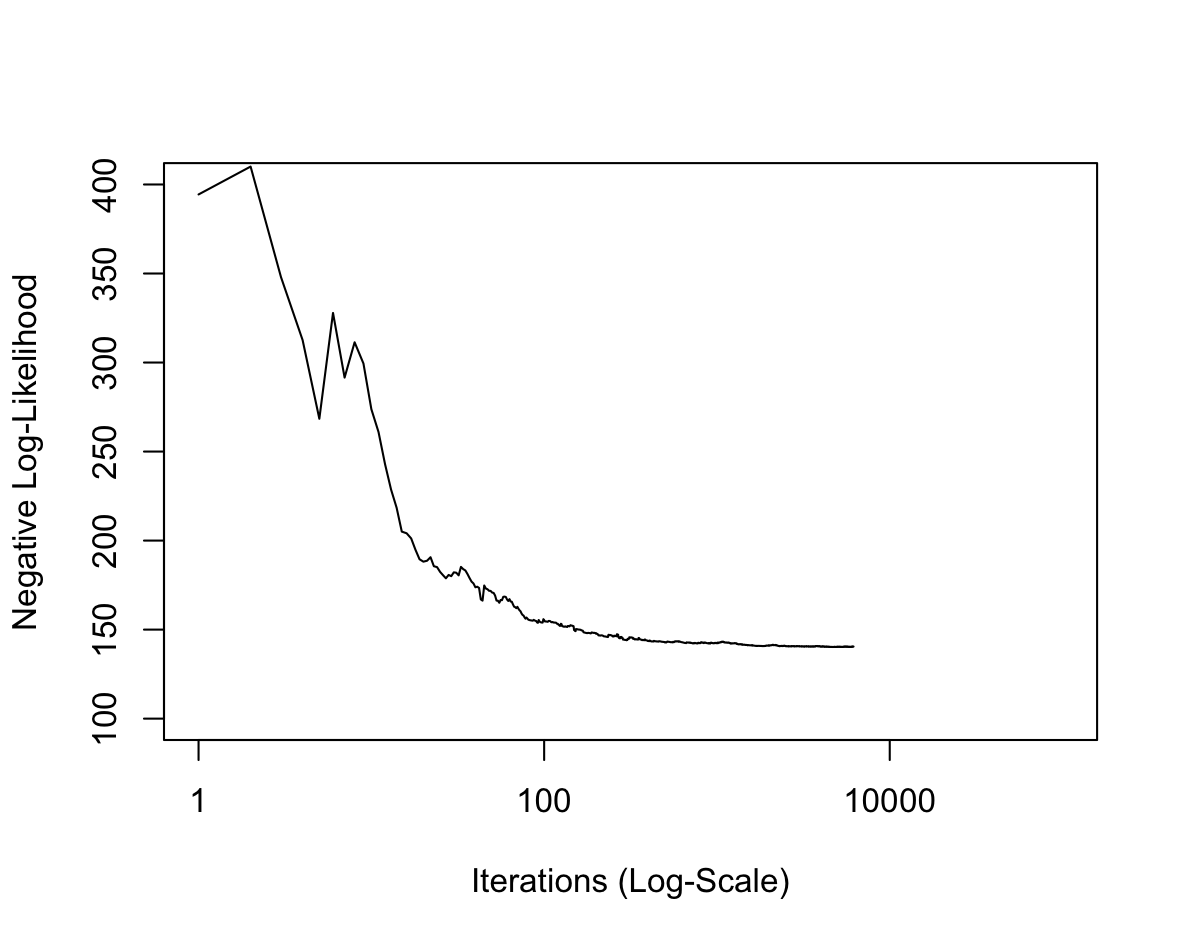
\includegraphics[width=\linewidth]{Fig/F2PD1.png}
				\caption{$C=1$}
			\end{subfigure}
			\caption{Decaying Step Size - experimenting with C ($t_0=1$ and $\alpha=0.6$)}
			\label{fig:Fig2}
		\end{center}
	\end{figure}

\begin{figure}[H]
	\begin{center}
		\begin{subfigure}[h]{0.45\linewidth}
			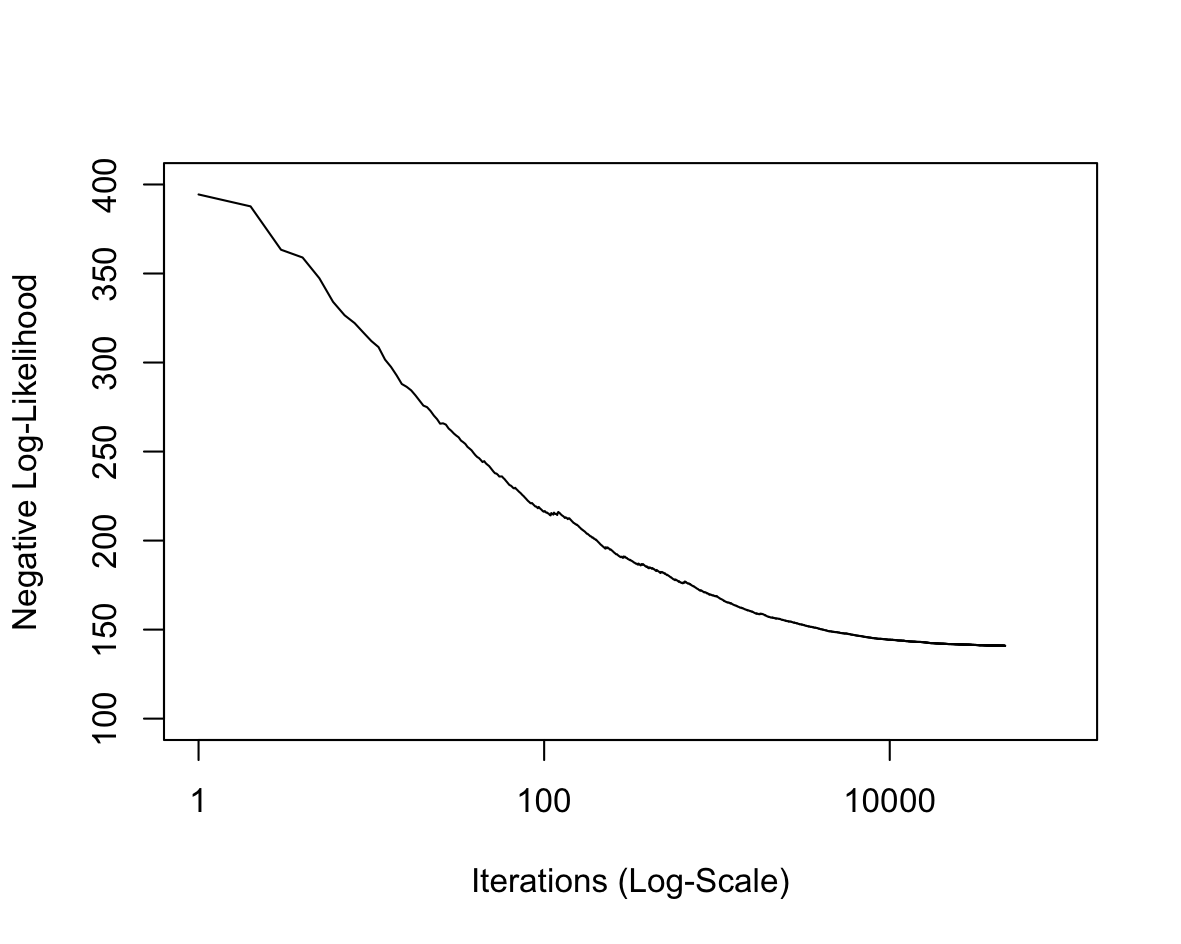
\includegraphics[width=\linewidth]{Fig/F3PD05.png}
			\caption{Learning rate $\alpha=0.5$}
		\end{subfigure}
		\begin{subfigure}[h]{0.45\linewidth}
			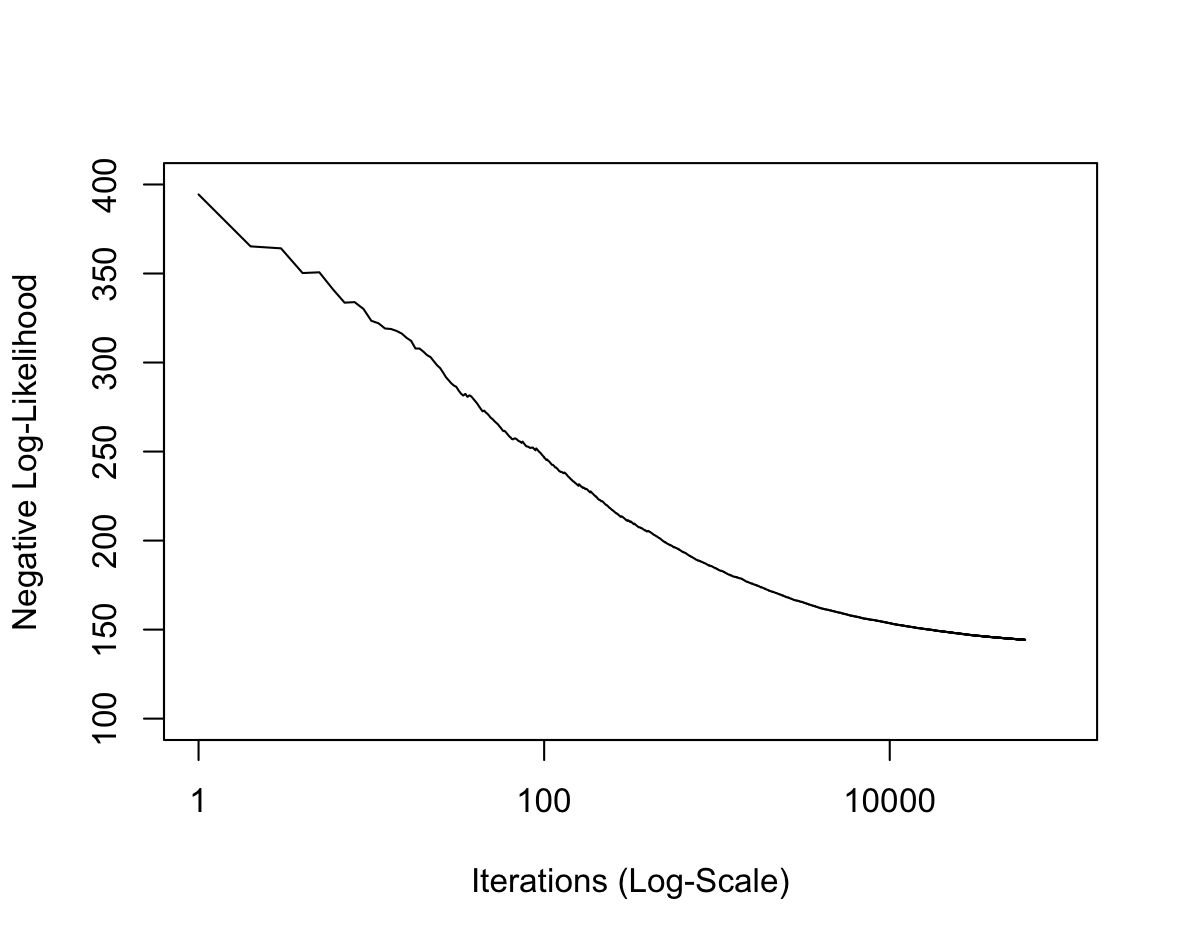
\includegraphics[width=\linewidth]{Fig/F3PD06.png}
			\caption{Learning rate $\alpha=0.6$}
		\end{subfigure}
		\begin{subfigure}[h]{0.45\linewidth}
			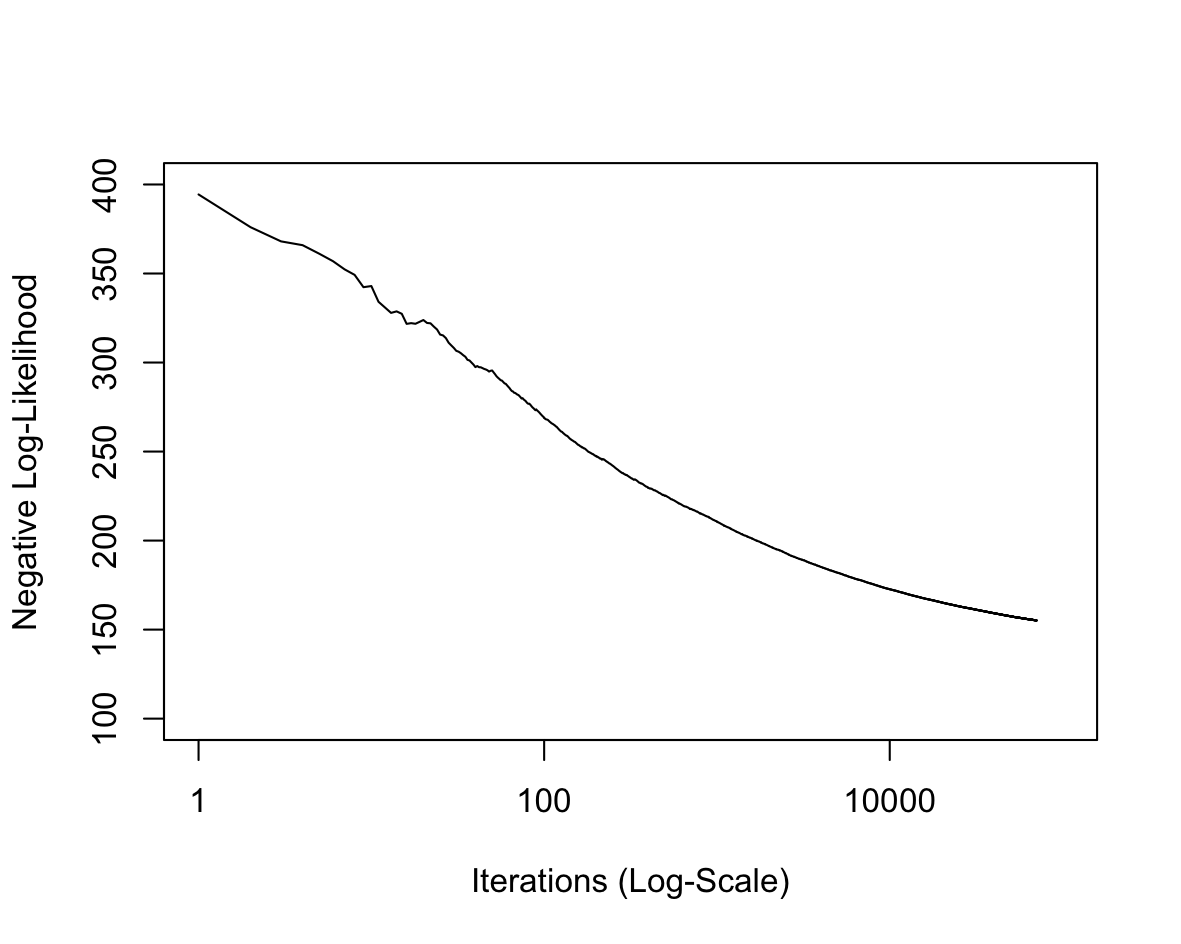
\includegraphics[width=\linewidth]{Fig/F3PD07.png}
			\caption{Learning rate $\alpha=0.7$}
		\end{subfigure}
		\begin{subfigure}[h]{0.45\linewidth}
			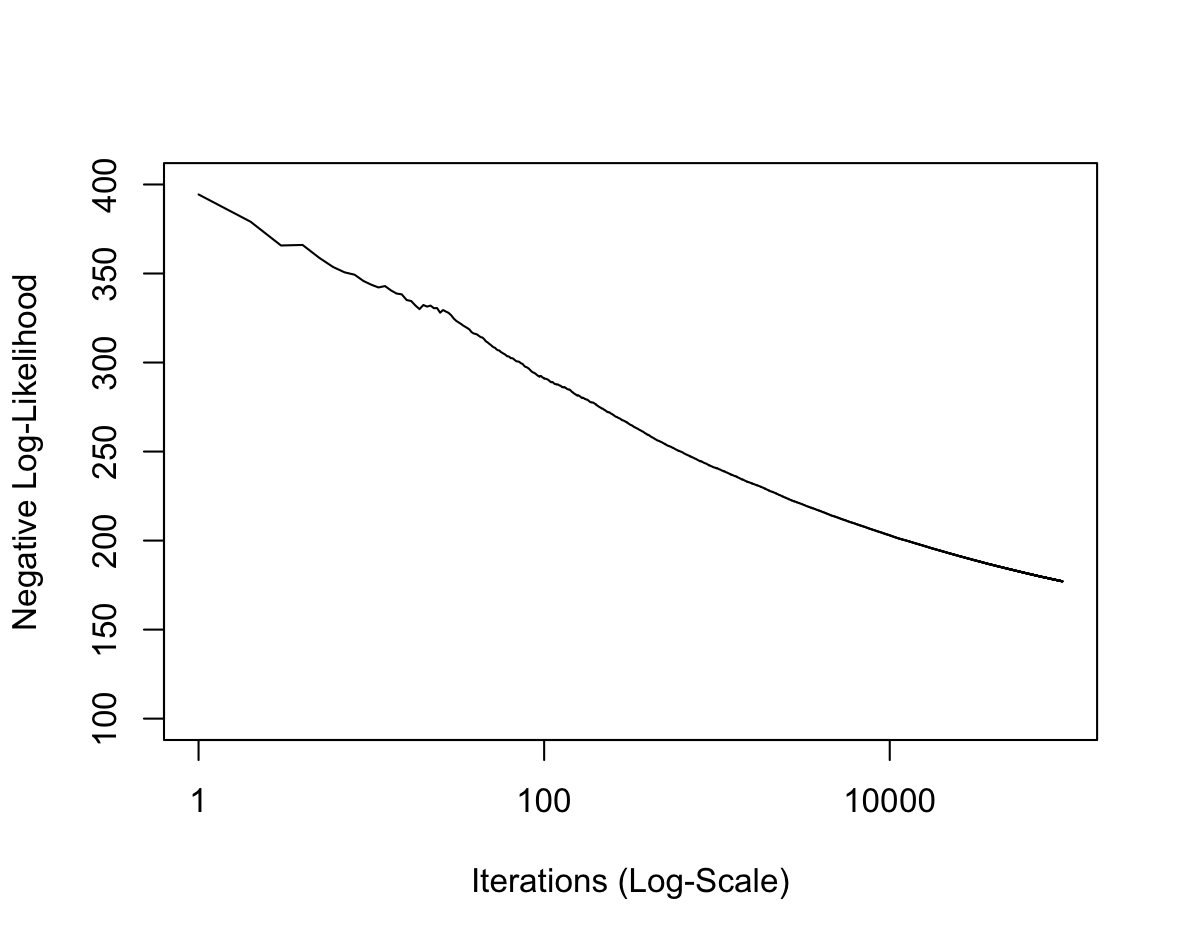
\includegraphics[width=\linewidth]{Fig/F3PD08.png}
			\caption{Learning rate $\alpha=0.8$}
		\end{subfigure}
		\begin{subfigure}[h]{0.45\linewidth}
			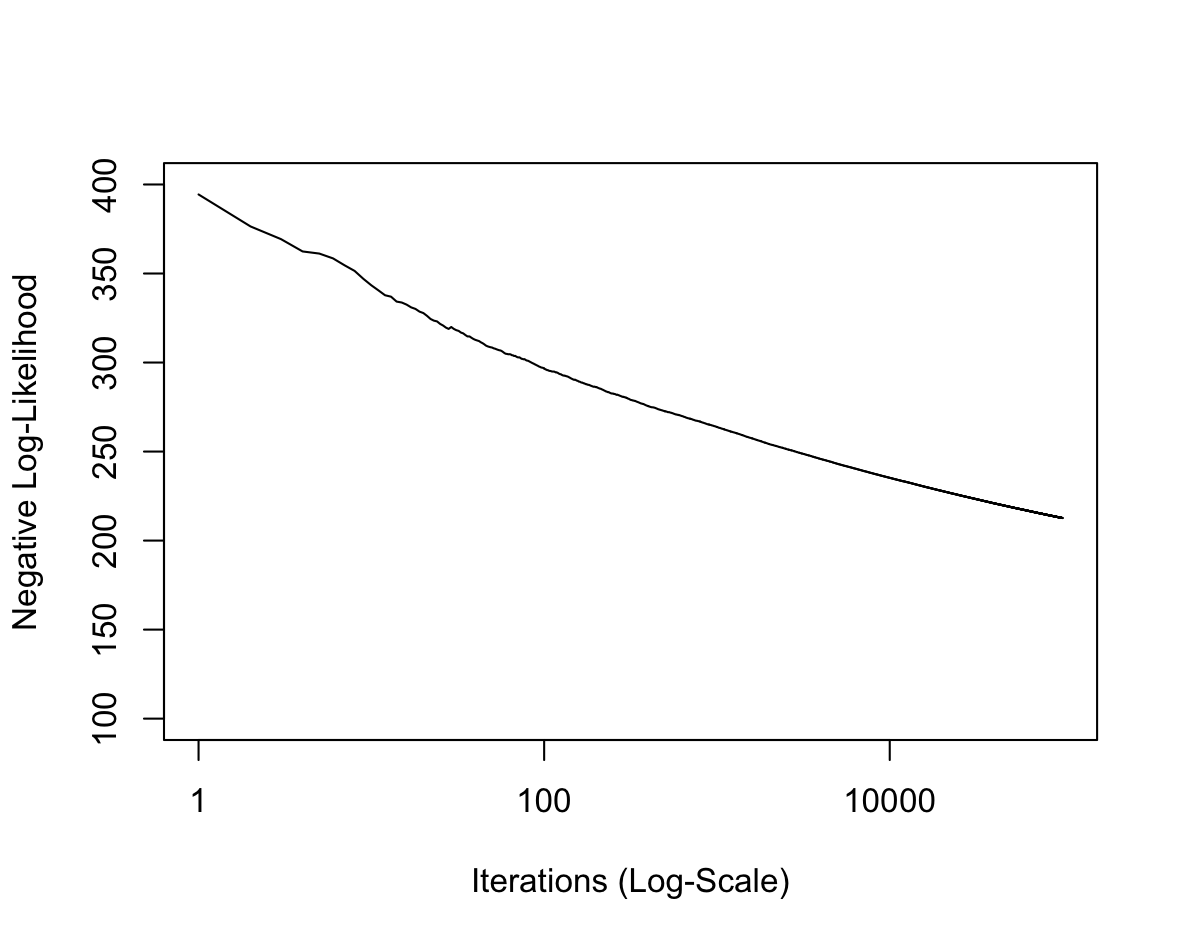
\includegraphics[width=\linewidth]{Fig/F3PD09.png}
			\caption{Learning rate $\alpha=0.9$}
		\end{subfigure}
		\begin{subfigure}[h]{0.45\linewidth}
			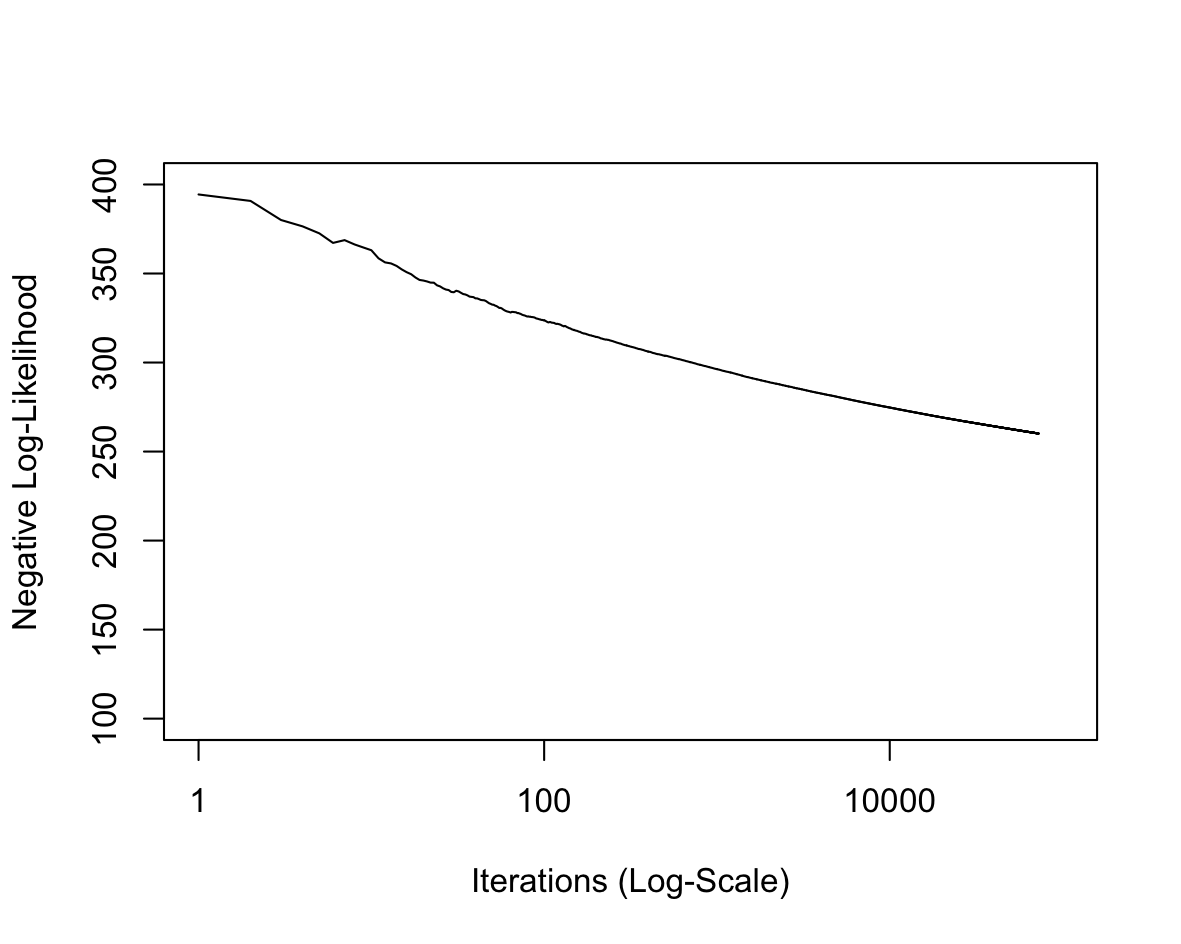
\includegraphics[width=\linewidth]{Fig/F3PD1.png}
			\caption{Learning rate $\alpha=1$}
		\end{subfigure}
		\caption{Decaying Step Size - experimenting with the learning rate $\alpha$ ($t_0=1$ and $C=0.1$)}
		\label{fig:Fig3}
	\end{center}
\end{figure}


\end{enumerate}


	
\end{document}